\documentclass[a4paper]{article}
% Русский язык
\usepackage[utf8]{inputenc}
\usepackage[russian]{babel}
% Математические символы и формулы
\usepackage{mathtools}
% Разбиение на разные файлы
\usepackage{subfiles}
% Отступы с краев(margin)
\usepackage[margin=1in]{geometry}
% Форматирование заголовков
\usepackage{titlesec}
\usepackage{indentfirst} % Красная строка
% Схемки
% \usepackage{circuitikz}
% Картинки
\usepackage{graphicx}

\begin{document}
\section{Способы записи функций алгебры логики}
\subsection{Таблица истиности}
\subsection{Описание ФАЛ в виде алгебраического выражения.}
По таблице истиности можно составить алгебраическое(булево) выражение. При этом запись алгебраического выражения осуществляется с использованием дизъюнктивной нормальной формы(ДНФ)
или конъюнктивной нормальной формы(КНФ)
Для представления логической функции $F$ в виде ДНФ необходимо составить сумму(дизъюнкцию)
произведений(конъюнкций) значений логической функции $F_i$ и минтернов $m_i$ т.е.
$$ F = \Sigma_{i = 1}^n (F_i * m_i) $$ Где $F$ - число строк в таблице истиности
Минтерм это логическое произведение всех переменных, причем переменные равные нулю записываются с инверсией.

\begin{table}[ht]
\centering
\begin{tabular}{|c|c|c|c|c|c|}
\hline
$x_3$ & $x_2$ & $x_1$ & $F$ & Минтерм & Макстерм \\
\hline
0 & 0 & 0 & 0 & $ m_1 = \neg x_3\neg x_2\neg x_1 $ & $ k_1 = x_3 + x_2 + x_1    $ \\
0 & 0 & 1 & 0 & $ m_2 = \neg x_3\neg x_2x_1  $ & $ k_2 = x_3 + x_2 + \neg x_1   $ \\
0 & 1 & 0 & 1 & $ m_3 = \neg x_3x_2\neg x_1  $ & $ k_3 = x_3 + \neg x_2 + x_1   $ \\
0 & 1 & 1 & 0 & $ m_4 = \neg x_3x_2x_1   $ & $ k_4 = x_3 + \neg x_2 + \neg x_1  $ \\
1 & 0 & 0 & 1 & $ m_5 = x_3\neg x_2\neg x_1  $ & $ k_5 = \neg x_3 + x_2 + x_1   $ \\
1 & 0 & 1 & 1 & $ m_6 = x_3\neg x_2x_1   $ & $ k_6 = \neg x_3 + x_2 + \neg x_1  $ \\
1 & 1 & 0 & 1 & $ m_7 = x_3x_2\neg x_1   $ & $ k_7 = \neg x_3 + \neg x_2 + x_1  $ \\
1 & 1 & 1 & 1 & $ m_8 = x_3x_2x_1    $ & $ k_8 = \neg x_3 + \neg x_2 + \neg x_1 $ \\
\hline
\end{tabular}
\end{table}

$$ F = m_1*0 + m_2*0 + m_3*1 + m_4*0 + m_5*1 + m_6*1 + m_7*1 + m_8*1$$

Для записи функции в дизъюнктивной нормальной форме можно использовать следующее правило следует записать столько дизъюнктивных членов, представляющих собой произведение всех переменных, сколько раз функция принимает значение единицы. Причем переменные равные нулю записываются с инверсией.

Для представления логической функции $F$ в виде конъюктивной нормальной формы необходимо составить произведение или конъюнкцию сумм или дизъюнкций и макстермов $k_i$. Причем число произведений равно числу строк в таблице истиности.
КНР

$$ F = \Pi_{i=1}^n (F_I + k_i) $$

Макстерм - логическая сумма всех переменных, причем переменные равные единице записываются с инверсией.

$$ F = (k_1 + 0) * (k_2 + 0) * (k_3 + 1) * (k_4 + 0) * (k_5 + 1) * (k_6 + 1) * (k_7 + 1) * (k_8 + 1)$$

Для записи функции в КНФ использую следующее правило. Следует записать столько конъюнктивных членов, представляющих собой дизъюнкции всех переменных, сколько раз функция принимает значение нуля. Причем переменные равные единице записываются с инверсией.

Должна быть реализована схема с тремя входами, которая на выходе выдает единицу тогда, когда четное число входных сигналов равно единице.
Или все сигналы равны нулю.

\begin{table}[ht]
\centering
\begin{tabular}{|c|c|c|c|}
\hline
$x_2$ & $x_1$ & $x_0$ & $F$ \\
\hline
0 & 0 & 0 & 1 \\
0 & 0 & 1 & 0 \\
0 & 1 & 0 & 0 \\
0 & 1 & 1 & 1 \\
1 & 0 & 0 & 0 \\
1 & 0 & 1 & 1 \\
1 & 1 & 0 & 1 \\
1 & 1 & 1 & 0 \\
\hline
\end{tabular}
\end{table}

ДНФ
Равны единице строчки: 0, 3, 5, 6
$$ F = (\neg x2\neg x1\neg x0) + (\neg x2\neg x1\neg x0) + (x2\neg x1x0) + (x2x1\neg x0)$$

$ x_2 $
$ x_1 $
$ x_0 $

% Схема 1


КНФ
Равны нулю строчки: 1, 2, 4, 8
$$ F = (x2+x1+\neg x0)*(x2+\neg x1+x0)*(\neg x2+x1+x0)*(\neg x2+\neg x1+\neg x0)$$


% Схема 2

\subsubsection{Описание ФАЛ в виде последовательности десятичных чисел}
Иногда для сокращения записи ФАЛ представляют в виде последовательно записаных десятичных эквивалентов двоичных кодов соответствующих конституант единице и нуля.

\begin{enumerate}
\item ДНФ
$$ F(x_2, x_1, x_0) = \Sigma(0, 3, 5, 6) $$
\item КНФ
$$ F(x_2, x_1, x_0) = \Pi(1, 2, 4, 7) $$
\end{enumerate}

\section{Комбинационные устройства}
Комбинационные устройства не имеют внутренней памяти.
Уровни их выходных сигналов всегда однозначно определяются текущими уровнями входных сигналов и никак не связаны с их предыдущими значениями.
Любое изменение входных сигналов обязательно изменяет состояние выходных.
Все комбинационные микросхемы построены из набора простейших логических элементов
\subsection{Мультиплексор}
Это комбинационное устройство, предназначенное для управляемой передачи данных от нескольких источников информации в один 
выходной канал.
Схематически мультиплексор можно предствить в виде многопозиционного ключа, обеспечивающего подключенние одного из нескольких входов(их называют информационными) к одному выходу устройства.
Кроме информационных входов в мультиплексоре имеются адресные входы и как правило разрешаюшие(или стробирующие).
Сигналы на адресных входах определяют какой конкретно информационный канал должен быть подключен к выходу.
Разрешающие входы используют для расширения функциональных возможностей мультиплексора.

\begin{enumerate}
    \item Наращивание разрядности мультиплексора
    \item Синхронизация его работы с работой других узлов
    \item Сигналы на разрешающих входах могут как разрешать, так и запрещать подключение определенного входа к выходу. Т.е. могут блокировать действие всего устройства.
\end{enumerate}
%Multisim

% Image of multiplexor
\begin{figure}[ht]
    \centering
    \includegraphics[width=\linewidth/3]{MUX.png}
    \caption{Мультиплексор. MUX(MS)}
\end{figure}

$$ n = 2^m $$
m - количество адресных входов
n - количество информационных входов

$ v = 0 $ => Работа устройства разрешена
$ v = 1 $ => Работа устройства запрещена

\begin{table}[ht]
\centering
\begin{tabular}{|c|c|c|c|}
\hline
$V$ & $A_1$ & $A_0$ & $Q$ \\
\hline
1 & * & * & 0 \\
0 & 0 & 0 & $I_0$ \\
0 & 0 & 1 & $I_1$ \\
0 & 1 & 0 & $I_2$ \\
0 & 1 & 1 & $I_3$ \\
\hline
\end{tabular}
\end{table}

$$Q = \neg A_1\neg A_0I_0 + \neg A_1A_0I_1 + A_1\neg A_0I_2 + A_1\neg _0I_3$$

%Схема 
\subsection{Демультиплексор}
Это устройство, в котором сигналы с одного информационного входа поступают в желаемой последовательности по нескольким выходам. В зависимости от входа на адресных шинах.

$$ n = 2^m $$

m - число адресных входов, n - число выходов.
DMX

\begin{table}[ht]
\centering
\begin{tabular}{|c|c|c|c|c|c|c|}
\hline
$V$ & $A_1$ & $A_0$ & $Y_0$ & $Y_1$ & $Y_2$ & $Y_3$\\
\hline
1 & * & * & 0 & 0 & 0 & 0 \\
1 & 0 & 0 & $D_I$ & 0 & 0 & 0 \\
1 & 0 & 1 & 0 & $D_I$ & 0 & 0 \\
1 & 1 & 0 & 0 & 0 & $D_I$ & 0 \\
1 & 1 & 1 & 0 & 0 & 0 & $D_I$ \\
\hline
\end{tabular}
\end{table}
    
$$ Y_0 = \neg A_0\neg A_1\neg VD_I $$
$$ Y_1 = A_0\neg A_1\neg VD_I $$
$$ Y_2 = \neg A_0A_1\neg VD_I $$
$$ Y_3 = A_0A_1\neg VD_I $$

\subsection{Шифратор}
Это комбинационное устройство преобразующее десятичные числа в двоичную систему счисления.

CD
\begin{figure}[ht]
    \centering
    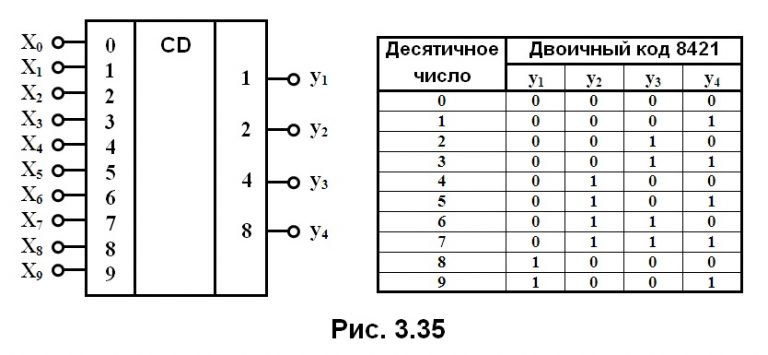
\includegraphics[width=\linewidth/3]{CD.jpg}
    \caption{Шифратор}
\end{figure}
% Таблица с двоичным кодом

$$ y_1 = x1 + x3 + x5 + x7 + x9 $$
$$ y_2 = x2 + x3 + x6 + x7 $$
$$ y_3 = x4 + x5 + x6 + x7 $$
$$ y_4 = x8 + x9 $$

\section{Последовательностные логические устройства}
Особенностью последовательностных логических устройств является зависимость выходного сигнала не только от действующих в настоящий момент на входе логических переменных, но и от тех значений переменных, которые действовали на входе в предыдущие моменты времени. 
\subsection{Триггеры}
Триггером называется устройство способное формировать два устойчивых значения выходного сигнала и скачкообразно изменять эти значения под действием внешнего управляющего сигнала.
Именно способность формировать на выходе два устойчивых значения сигнала, которые могут поддерживаться без изменения сколь угодный длительный промежуток времени и позволяет применять триггер в качестве элемента памяти. 

Входы триггеров разделяют на информационные и управляющие. Информационные входы используются для управления состояниями триггера. управляющие входы используются для предварительной установки триггера в некоторое состояние и для синхронизации.
Триггеры бывают ассинхронные и синхронные(синхронные статические и синхронные динамические)

Ассинхронный триггер изменяет свое состояние непосредственно в момент появления соответствующего информационного сигнала

и-не/или-не
Ассинхронный $RS$-триггер построенный на элементах или-не 

Set - вход установки
Reset - сброс

Управляющим сигналом для $RS$-триггера построенного на элементах или/не является логическая единица.

\begin{table}[ht]
\centering
\begin{tabular}{|c|c|c|c|c|}
    \hline
    $S$ & $R$ & $Q$ & $\not Q$ & описание \\
    \hline
    1 & 0 & 1 & 0 & установка\\
    0 & 0 & 1 & 0 & хранение\\
    0 & 1 & 0 & 1 & сброс \\
    0 & 0 & 0 & 1 & хранение \\
    1 & 1 & - & - & запрещенная операция \\
    \hline
\end{tabular}
\end{table}

Ассинхронный $RS$-триггер построенный на элементах и-не 
Управляющим сигналом для $RS$-триггера построенного на элементах и/не является логический ноль.

\begin{table}[ht]
\centering
\begin{tabular}{|c|c|c|c|c|}
    \hline
    $S$ & $R$ & $Q$ & $\not Q$ & описание \\
    \hline
    0 & 1 & 1 & 0 & установка\\
    1 & 1 & 1 & 0 & хранение\\
    1 & 0 & 0 & 1 & сброс \\
    1 & 1 & 0 & 1 & хранение \\
    0 & 0 & - & - & запрещенная операция \\
    \hline
\end{tabular}
\end{table}

Синхронные триггеры реагируют на информационные сигналы только при наличии соответствующего сигнала на так называемом входе синхронизации $C(clock)$

\subsection{Синхронные статические триггеры}
Статические триггеры воспринимают информационные сигналы при подаче на вход $C$ логической единице или либо логического нуля.

Синхронный статический $RS$-триггер на элементах и-не

\begin{table}[ht]
\centering
\begin{tabular}{|c|c|c|c|c|}
    \hline
    $C$ & $S$ & $R$ & $Q$ & описание \\
    \hline
    0 & 1 & 0 & 1 & хранение\\
    1 & 1 & 0 & 1 & установка \\
    1 & 0 & 1 & 0 & сброс \\
    0 или 1 & 1 & 1 & 0 & хранение \\
    1 & 0 & 0 & - & запрещенная операция \\
    \hline
\end{tabular}
\end{table}

\subsection{Синхронный статический JK-триггер}

JK-триггер управляется логической единицей и не имеет запрещенных комбинаций для входных сигналов.

\begin{table}[ht]
\centering
\begin{tabular}{|c|c|c|c|c|}
    \hline
    $J$ & $K$ & $C$ & $Q$  & описание \\
    \hline
    1 & 0 & 1 & 1 & установка\\
    0 & 1 & 0 & 1 & хранение \\
    0 & 1 & 1 & 0 & сброс \\
    0 & 0 & 0 или 1 & 0 & хранение \\
    1 & 1 & 1 & 1 & инверсия выходного сигнала \\
    1 & 1 & 1 & 0 & инверсия выходного сигнала \\
    \hline
\end{tabular}
\end{table}

Синхронный статический $D$-триггер
Хранение информации в $D$-триггерах обеспечивается за счет синхронизации поэтому все реальные D-триггеры имеют два входа: информационный $D$ и синхронизации $C$. В этом триггере сигнал на входе по приходу синхронизации записывается и передается на выход.

Информация на выходе остается неизменной до прихода очередного импульса синхронизации. 

\begin{table}[ht]
\centering
\begin{tabular}{|c|c|c|c|}
    \hline
    $C$ & $D$ & $Q$  & описание \\
    \hline
    1 & 1 & 1 & установка\\
    0 & 0 & 1 & хранение \\
    1 & 0 & 0 & сброс \\
    \hline
\end{tabular}
\end{table}
\end{document}

\subsection{Синхронные динамические триггеры}
Синхронные динамические триггеры воспринимают информационные сигналы при изменнении сигнала на входе $C$
от нуля к единице(прямой динамический вход синхронизации) или от единицы к нулю(инверсный динамический вход синхронизации).

Синхронный динамический $D$-триггер. 

\subsection{Т-триггер}

Может быть построен на основе D-триггера или на основе JK-триггера.